\datos{color}{}{}
\section{Enunciado}
%\addcontentsline{toc}{section}{Ejercicio 1}
En este tema se plantea un único ejercicio de investigación cuyo objetivo es clasificar
diversos tipos de robots de acuerdo a los conceptos introducidos en el desarrollo teórico
del tema. \\

El trabajo consiste en la búsqueda por medio de internet u otras fuentes de información
de al menos un ejemplo real de robot de cada uno de los tipos y arquitecturas mostrados
en la teoría. \\

De este modo deberá haber al menos un robot que tenga una arquitectura centralizada,
un robot con arquitectura distribuida y otro con arquitectura híbrida. Además tendrá que
haber al menos un robot con ruedas, un robot con cadenas, un robot con patas y un robot
marino o aéreo. También deberá ponerse algún ejemplo de robot colaborativo o de red
de sensores. \\

Para facilitar la corrección y la verificación por parte del alumno de que se están
cubriendo todos los tipos y arquitecturas debe rellenarse una tabla de la forma siguiente, 
Figura \ref{fig:tablaEnunciado}.

\begin{figure}[htb]
    \centering
    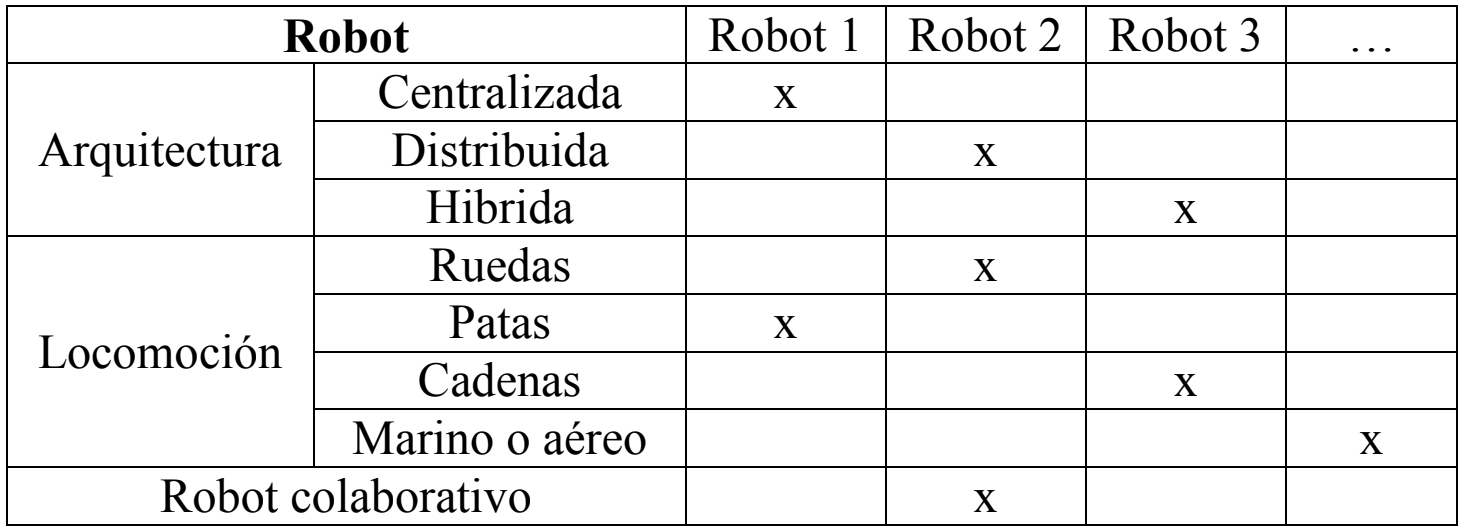
\includegraphics[scale=0.29]{Images/tablaEnunciado.png}
    \caption{Tabla a rellenar} \label{fig:tablaEnunciado}
\end{figure}

Para cada uno de los robots habrá que completar una pequeña ficha que contenga la
siguiente información.
\begin{itemize}
    \item Nombre.
    \item Breve descripción del robot.
    \item Uso(s) principal(es) del robot.
    \item Breve descripción de la arquitectura del robot.
    \item Breve descripción del método de locomoción.
    \item Empresa, entidad u organismo que lo ha construido.
    \item Fotografía del robot.
    \item Referencias (URLs o Referencias a libros o revistas donde pueda verificarse tal
información). \\
\end{itemize}

La ficha del robot no pretende ser una descripción exhaustiva, puesto que lo que se
pretende es comprobar que se han comprendido correctamente los tipos de robots y
arquitecturas existentes. Por este motivo el espacio destinado a la ficha de cada robot no
debe exceder una cara.